\documentclass{article}
\usepackage{amsmath}
\usepackage{amssymb}
\usepackage{graphicx}

\begin{document}


\renewcommand{\figurename}{Figura}

\center
\textbf{Problema del empaquetamiento de texturas}

\bigskip

\textbf{Integrantes:} 

Alejandro García González \quad \textbf{C411} 

Carlos Mauricio Reyes Escudero \quad \textbf{C411}

\bigskip
\bigskip

\textbf{0. Introducción}

\raggedright

La compresión de información es y siempre será un problema importante en computación. Si bien cuando el tamaño del almacenamiento o la velocidad de la red aumentan es posible manejar mayor cantidad de información, y más rápido, es difícil pensar que no aparecerá eventualmente un problema que pruebe los límites de la tecnología. En este trabajo nos centraremos en un caso particular de compresión: el empaquetamiento de texturas; esto es: dado un conjunto de imágenes, encontrar la mejor forma de compilarlas todas en una sola imagen. Un uso práctico de esto se encuentra en las tarjetas gráficas: convencionalmente las tarjetas gráficas tienen un número limitado (alrededor de 32) de los llamados ``texture slots", que no son más que trozos de memoria de tamaño fijo destinados a guardar texturas; es entonces conveniente agrupar múltiples texturas en un solo texture slot, lo que además reduce la cantidad de cambios de estado interno de la GPU (cambiar de una textura a otra), y aumenta la localidad espacial.

\bigskip

\center
\textbf{1. Demostrando que el problema es NP-Duro}

\raggedright
\smallskip

En esta sección demostraremos que un caso específico del problema es NP-Duro. Nos centraremos en cuando ``mejor forma" se refiere a empacar imágenes en una sola imagen padre minimizando el área, y en particular cuando el ancho de la imagen padre es fijo. Formalizando: 

\bigskip

\textbf{Definición} (Strip Packing problem): Dado un conjunto de rectángulos (con lados alineados a los ejes), y un ancho fijo $W$, hallar la mínima altura $H$ para la cual se pueden empacar sin solapamiento todos los rectángulos del conjunto en un rectángulo de $W \times H$.

\bigskip

A continuación mencionamos la cadena de reducciones que seguiremos para demostrar que nuestro problema es difícil. La notación $Y \leq_p X$ significa ``el problema Y se reduce polinomialmente al problema X".
\bigskip

\small{3-SAT $\leq_p$ 3D-Matching $\leq_p$ 4-Partition $\leq_p$ Rectangle Packing $\leq_p$ Strip Packing}

\bigskip

\textbf{Definición} (3D-Matching problem): Dado 3 conjuntos $X$, $Y$ y $Z$ disjuntos, cada uno de tamaño $n$, y un conjunto de triplas $T \subseteq X \times Y \times Z$, determinar si existe un $S \subseteq T$ tal que para todo $e \in X \cup Y \cup Z$, $e$ aparece en exactamente una tripla $s \in S$.

\smallskip

Informalmente: Dado una especie de ``grafo" donde las ``aristas" conectan a 3 nodos entre sí en lugar de solo a 2, y que es tripartito, hallar un ``emparejamiento" (entriplamiento?) perfecto.

\bigskip
\textbf{Teorema:} 3D-Matching es NP-Completo.

\smallskip

\textbf{Demostración:}

\bigskip

Es fácil ver que dado un conjunto de triplas, se puede comprobar en tiempo polinomial que dicho conjunto da un 3D-Matching completo válido. O sea, 3D-Matching $\in$ NP.

\bigskip

Ahora, para demostrar que es NP-Duro, reduzcamos 3-SAT a 3D-Matching. Dada una formula booleana en forma normal conjuntiva, hagamos lo siguiente:

\begin{figure}[hp]
	\begin{center}
		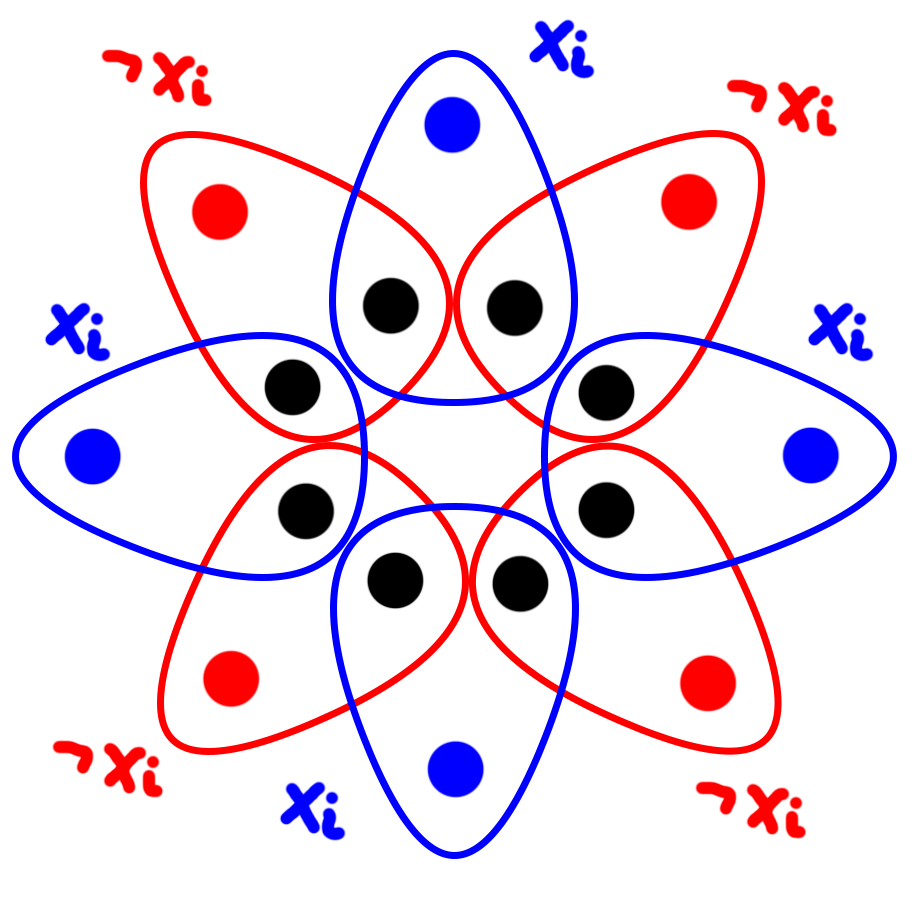
\includegraphics[scale=0.2]{IMGs/3DM 1.png}	
	\end{center}
\end{figure}

Por cada variable que aparece en la fórmula, construyamos un gadget como el que aparece en la figura. Este tiene el nombre de ``gadget variable". Que 3 nodos estén encerrados dentro de un óvalo significa que están conectados entre sí (o sea, los óvalos son las ``aristas" de esta especie de ``grafo"). Pero la cantidad de picos del gadget será $2n_{x_i}$, donde $n_{x_i}$ es la cantidad de veces que aparece la variable $x_i$ (o su negación) en la fórmula. Este gadget tiene la peculiaridad de que los nodos que se muestran en negro no están conectados con nada fuera del gadget (se verá que los rojos y azules sí). Esto implica que para lograr un 3D-Matching perfecto, es necesario matchearlos utilizando los óvalos del gadget. Se comprueba entonces que para poder seleccionar a todos los nodos negros, hay solo dos posibilidades: o se eligen solo los óvalos azules o solo los rojos para estar en el matching (cualquier combinación de rojos y azules poseería solapamiento). Esto corresponde a elegir verdadero o falso para la variable $x_i$. En particular: si se escogen solo los óvalos rojos, o sea que se dejan libres los azules, esto correspondería a elegir verdadero para la variable; y viceversa si se escogen los azules. Esto es así porque dejar nodos libres permite a otros gadgets usarlos, como se verá a continuación.

\pagebreak

\begin{figure}[hp]
	\begin{center}
		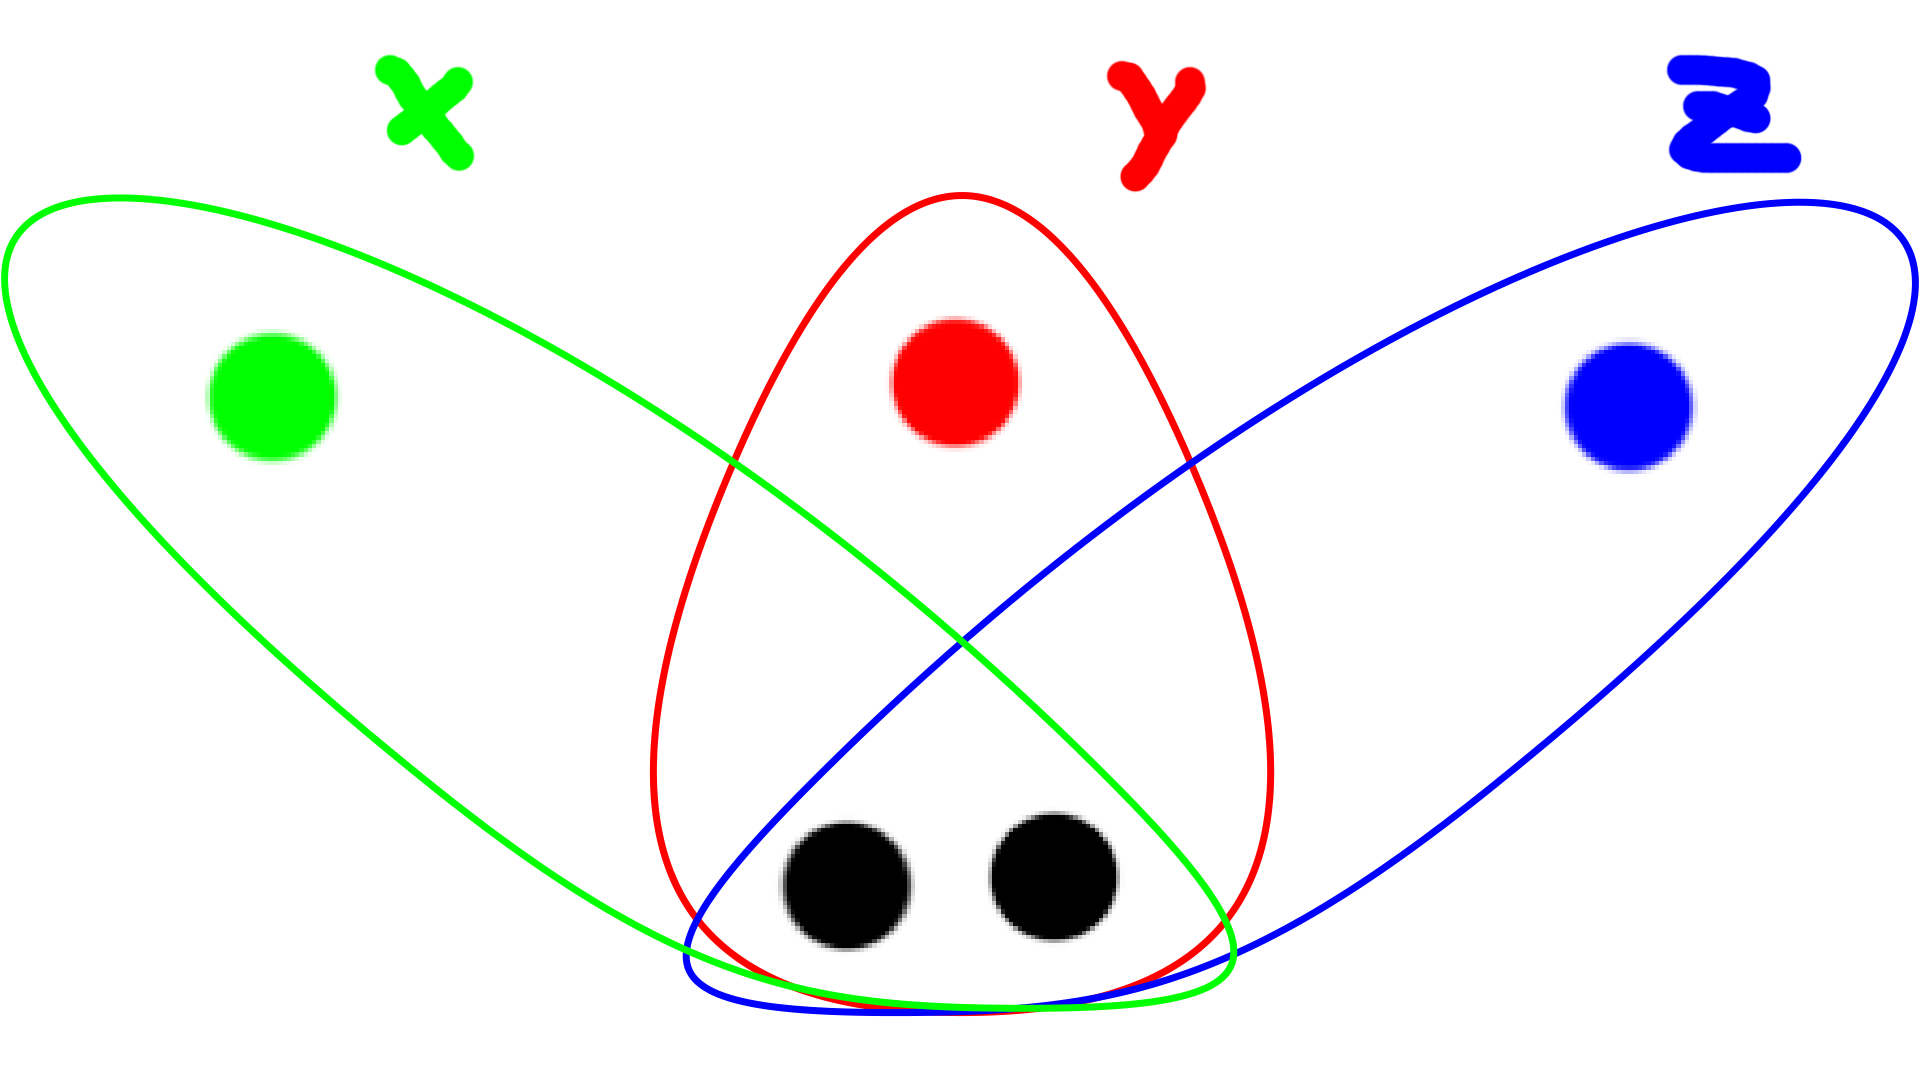
\includegraphics[scale=0.1]{IMGs/3DM 2.png}	
	\end{center}
\end{figure}

Por cada cláusula $(x \vee y \vee z)$, hagamos la construcción que se muestra en la figura. Los nodos negros son locales (no están conectados a más nada fuera del gadget), pero los de colores son los exteriores de uno del gadget correspondiente a las variables x, y, z respectivamente (nos aseguramos anteriormente de que cada gadget variable tuviera suficientes picos para poder hacer esto sin solapamiento). Como en el gadget variable, si se quiere lograr un 3D-Matching perfecto, los nodos negros se tienen que matchear usando alguno de los óvalos del gadget (que por cierto, recibe el nombre de ``gadget cláusula"). Esto corresponde a satisfacer esta cláusula usando el valor de una de sus variables. Entonces, satisfacer la fórmula sería equivalente a satisfacer todos los gadget cláusula. 

\bigskip

Falta un detalle. Si la operación de dentro de una cláusula fuera un XOR en lugar de un OR, ya estaría la demostración terminada. Pero en una cláusula puede haber más de una variable satisfecha. Así que queda poner un ``parche" para cuando esto pasa.




\begin{figure}[hp]
	\begin{center}
		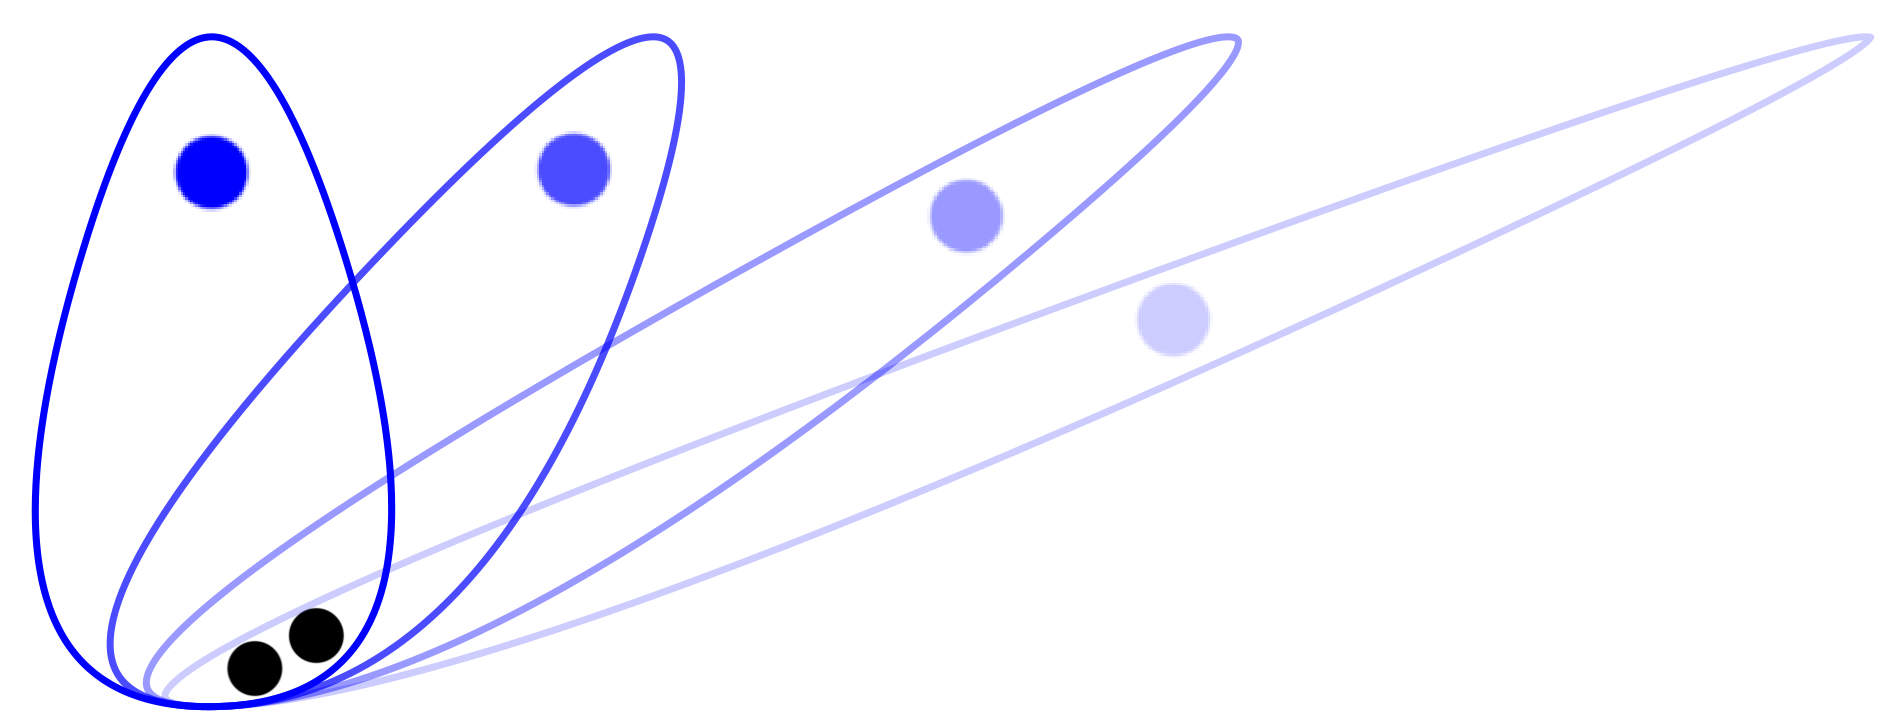
\includegraphics[scale=0.1]{IMGs/3DM 3.png}	
	\end{center}
\end{figure}


Creamos así un tercer y último gadget, que le llamaremos ``gadget recolector de basura". Este consistirá en dos nodos locales (de nuevo los nodos negros de la figura), los que estarán conectados a todos los otros nodos pico de los gadgets variables. De esta forma, los nodos que ``sobren" (o sea, que se hayan dejado libre en su gadget variable, y no se hayan usado para satisfacer algún gadget cláusula), se matchearán acá. La idea es usar $\sum{n_{x_i}} - \#clauses$ de estos gadgets, es decir, asumiendo que se hayan satisfecho todas las cláusulas, uno por cada nodo que se dejó sin matchear.

\bigskip

De esta forma ya tenemos una instancia (de tamaño polinomial) del problema de 3D-Matching que retorna verdadero ssi la fórmula que nos pasaron es satisfacible. $\blacksquare$

\bigskip

\textbf{Definición} (4-Partition problem): Dado un conjunto de $n$ enteros $A = \{ a_1, ..., a_n \}$, determinar si existe una partición del conjunto en $n/4$ subconjuntos, de 4 elementos cada uno, con la misma suma (que resulta tener que ser necesariamente $t = \frac{\sum A}{n/4}$).

\bigskip

\textbf{Teorema:} 4-Partition es NP-Completo.

\smallskip

\textbf{Demostración:}

\bigskip

Está claro que si se tiene una partición, comprobar que es válida es fácil: se suman los 4 números de cada subconjunto por separado, y se comprueba que todos den la misma suma. Luego, 4-Partition $\in$ NP.

\bigskip

Ahora, para demostrar que es NP-Duro, reduzcamos 3D-Matching a él. Entonces, dada una entrada al 3D-Matching, hagamos la siguiente construcción:

\bigskip

Vamos a llenar el conjunto que se quiere particionar para resolver el 3D-Matching con el 4-Partition. Procederemos a escribir los números en una especie de representación en base $r$, para un $r$ lo suficientemente grande (para poder razonar mayormente dígito a dígito). En particular, usaremos $r = 100 \times 3n$, donde $n$ es el tamaño de cada conjunto del 3D-Matching. En lo siguiente, la notación $(a,b,c,d,e)$ representará al número $ar^4+br^3+cr^2+dr+e$. En un momento usaremos ``dígitos negativos", lo que justificaremos luego. Ahora, listemos por cada conjunto y tripla del 3D-Matching, qué números añadimos al conjunto a particionar, y cuál sería la suma objetivo (dictada por la estructura del conjunto, claro) y luego justifiquemos por qué resolver el 4-Partition en dicho conjunto es equivalente a resolver el 3D-Matching. 

\bigskip
Por cada $x_i \in X$ $\rightarrow$ $(10, i, 0, 0, 1)$ y $(11, i, 0, 0, 1)$ $\times$ ($n_{x_i} - 1$) copias

Por cada $y_j \in Y$ $\rightarrow$ $(10, 0, j, 0, 2)$ y $(11, 0, j, 0, 2)$ $\times$ ($n_{y_j} - 1$) copias

Por cada $z_k \in Z$ $\rightarrow$ $(10, 0, 0, k, 4)$ y $(8, 0, 0, k, 4	)$ $\times$ ($n_{z_k} - 1$) copias

Por cada tripla ($x_i$, $y_j$, $z_k$) $\rightarrow$ $(10, -i, -j, -k, 8)$ 

Suma objetivo (se demostrará en breves) $\rightarrow$ $t = (40, 0, 0, 0, 15)$

\bigskip

Ahora a demostrar. Primero, demostremos que la suma es la suma objetivo es la que decimos allá arriba. La suma de cada subconjunto debe ser la suma total sobre un cuarto de la cantidad de elementos del conjunto. La cantidad de elementos del conjunto es $4 \times \#triplas$, ya que por cada tripla hay un elemento que la representa, y por cada número de la tripla hay un elemento que lo representa; o sea, cada tripla se cuenta otras 3 veces. La suma total del conjunto se halla sumando dígito a dígito. Esta termina siendo $(40r^4+15)\times \#triplas$. Dividiendo, queda demostrado que la suma es t.

\bigskip

Es importante justificar el uso de esos ``dígitos negativos". Si bien en el contexto tienen sentido (no son más que coeficientes en una suma ponderada de potencias de $r$), en nuestro caso nos conviene que no interfieran con el dígito menos significativo, o sea, que independientemente de los valores de $i$, $j$ y $k$, el valor del dígito menos significativo sigue siendo 8. Para esto, basta con que $10r^4-ir^3-jr^2-kr \geq 0$ para los valores máximos de $i$, $j$ y $k$, que son en los tres casos n (el tamaño de cada conjunto del 3D-Matching). Esto se logra sustituyendo el valor de $r$ en función de $n$ en esa expresión ($r = 3 \times 10^2 \times n$), sustituyendo $i$, $j$ y $k$ por su valor máximo $n$; luego de esto se reduce la expresión a una cuadrática con coeficiente principal positivo y ceros estrictamente menores a 1, lo que demuestra que la inecuación se cumple para todo valor de $n$, y por tanto para todo valor posible de $i$, $j$, $k$ y $r$. 

\bigskip

Ahora la pieza final de la demostración. Como la única forma de formar $15$ sumando cuatro potencias de $2$ es $8+4+2+1$, y el dígito menos significativo es independiente, entonces para formar un cuarteto de números que sumen a $t$ es necesario tomar uno que haya sido generado por el conjunto $X$, uno por el conjunto $Y$, uno por el $Z$ y uno por una tripla. Al sumar un elemento generado por cada uno de $X$, $Y$ y $Z$, los dígitos del medio quedan $(i,j,k)$, por lo que hay que sumar el elemento generado por la tripla hay que cancelarlos, lo que implica que hay que sumar el elemento de la tripla $(i,j,k)$. Por último, hay dos maneras de llegar a 40: sumando los 3 elementos únicos generados por cada conjunto (aquellos de dígito más significativo 10) junto a su tripla correspondiente, o sumando los elementos de los que se generan varios por nodo (dígito menos significativo 11, 11, 8, que cumplen $11+11+8=30$) junto a la tripla correspondiente.  La primera alternativa corresponde a tomar la tripla $(i,j,k)$ dentro del Matching, la segunda a no tomarla. Entonces, habrá 3D-Matching Perfecto ssi hay una forma de agrupar todos los elementos únicos generados por $X$, $Y$ y $Z$, con una tripla correspondiente. $\blacksquare$

\bigskip

\textbf{Definición} (Rectangle Packing problem): Dado un conjunto de rectángulos (con lados alineados a los ejes), y un rectángulo más grande (también con lados alineados a los ejes) cuya área es la suma de las áreas de dichos rectángulos, determinar si es posible cubrir completamente el rectángulo grande con los otros sin solapamiento. No se permite rotar ningún rectángulo.

\bigskip

\textbf{Teorema:} Rectangle Packing es NP-Completo.

\smallskip

\textbf{Demostración:}

\bigskip

Si se tiene la posición de cada rectángulo pequeño, es fácil comprobar en tiempo polinomial que no haya solapamiento (basta con comprobar intersección entre todo par de rectángulos), y si no hay solapamiento, como la suma de sus áreas es igual a la del rectángulo grande, entonces dicho rectángulo está completamente cubierto. Luego, Rectangle Packing $\in$ NP.

\bigskip

Para demostrar que es NP-Duro, reduzcamos 4-Partition a él. Esta reducción es relativamente sencilla: convertimos cada elemento $a_i$ del conjunto que se quiere particionar en un rectangulito de $a_i \times 1$, y ponemos que nuestro rectángulo base sea de $\frac{\sum A}{n/4} \times n/4$. Así cada fila del rectángulo grande representará un subconjunto, habiendo $n/4$ filas. $\blacksquare$

\bigskip

\textbf{Teorema:} Strip Packing es NP-Duro.

\smallskip

\textbf{Demostración:}

\bigskip

Reduzcamos Rectangle Packing a Strip Packing. Para resolver Rectangle Packing para un conjunto $R$ de rectángulos y un rectángulo grande de $W \times H$, basta con usar un algoritmo para Strip Packing, pasándole $R$ y $W$; si la salida de este algoritmo es $H$, existe un empaquetamiento perfecto (sin huecos), por lo que la respuesta a Rectangle Packing es True; si es distinta de $H$, tiene que ser estrictamente mayor que $H$, lo que significa que no es posible empaquetar los rectángulos de $S$ sin solapamiento en un rectángulo de $W \times H$, por lo que la respuesta a Rectangle Packing es False. $\blacksquare$



\bigskip

\center
\textbf{2. Una solución exacta}

\raggedright
\smallskip

Demostrado que el problema es NP-Duro, exploremos una alternativa para resolverlo exactamente que funciona bien en la práctica (o al menos, es de lo mejor que se puede hacer para resolver el problema exactamente). El algoritmo consistirá básicamente en reducir el problema a uno de programación en enteros, problema el cual es NP-Duro también, pero se conocen algoritmos prácticos para su resolución.

\bigskip

Asumiremos, sin pérdida de generalidad, que la entrada al algoritmo consiste en un conjunto de rectángulos $(w_i, h_i)$, cada uno de los cuales está repetido $d_i$ veces (o sea, hay exactamente $d_i$ rectángulos de tamaño $(w_i, h_i)$, están agrupados por tamaño), y el ancho fijo $W$ del rectángulo grande. Lo primero que hará el algoritmo es calcular una cota mínima para H. En la práctica se utiliza a menudo el área total de los rectángulos sobre el ancho del rectángulo grande. Esto es: asumiendo que el empaquetamiento quede perfecto (sin huecos, sin espacio desperdiciado), ¿cuál sería H?. Formalmente, la cota es:


\begin{flalign*}
	& H \geq \left \lceil{\frac{\sum d_iw_ih_i}{W}}\right \rceil  &
\end{flalign*}

Ahora, comenzando con este valor menor que $H$, y mientras no se haya hallado el $H$ óptimo, se realiza un proceso para ver si el $H$ actual es el óptimo. Describamos este proceso.

\bigskip

Por conveniencia, enumeremos linealmente los píxeles de la imagen grande, comenzando por uno en la esquina superior izquierda y terminando por $W \times H$. Ahora, por cada imagen pequeña $i$, haremos una tabla $C^i = c^i_{jp}$. Cada fila corresponderá a una posición válida de la imagen, es decir, a un pixel en el que poner la esquina superior izquierda de la imagen tal que dicha imagen no se pase de los límites de la imagen padre, y habrá una columna por cada pixel de la imagen padre, de forma tal que el elemento $c^i_{jp}$ es $1$ si para la imagen $i$, y la $j$-ésima posición válida de la esquina superior izquierda ($V[j]$), la imagen ocupa el pixel $p$, y en caso contrario $0$.

\bigskip

Ahora la formulación lineal del problema. Llamaremos a las variables de decisión $x_{ij}$, y tendremos una por cada imagen $i$, y cada posición válida $j$ de su esquina superior izquierda; así, $x_{ij} = 1$ si se decide que la imagen $i$ se debe posicionar en su  $j$-ésima posición válida $V[j]$, y 0 en otro caso. Entonces, sea $P$ el conjunto de posiciones de la imagen grande, $I$ el conjunto de imágenes, y $F^i$ el conjunto de las filas de la tabla de la imagen $i$, las restricciones a satisfacer son las siguientes:

\begin{flalign*}
	&\sum\limits_{i \in I} \sum\limits_{j \in F^i} c^i_{jp} x_{ij} \leq 1 \;\;\;\;\; \forall p \in P&
\end{flalign*}

\begin{flalign*}
	&\sum\limits_{j \in F^i} x_{ij} = d_{i}  \;\;\;\;\; \forall i \in I&
\end{flalign*}

\bigskip

La primera restricción garantiza que por cada pixel de la imagen padre, haya a lo sumo una imagen ocupándolo. La restricción se lee: ``por cada pixel $p$ de la imagen grande, pon un contador en cero, itera por todas las imágenes, y si para alguna posición válida de la esquina superior izquierda escogida de dicha imagen se usa el pixel $p$, suma uno al contador; para todos los casos el contador debe ser menor o igual a 1". 

\bigskip

La segunda restricción es más sencilla, está ahí para que la cantidad de imágenes del mismo tamaño que se pongan sea la correcta. Resulta que tratar a las imágenes del mismo tamaño en batch ayuda al algoritmo a converger. En la misma línea, se pueden añadir otras restricciones para ayudar al algoritmo, en las que no entraremos. 

\bigskip

La complejidad del algoritmo sería $O(\, H \cdot ((HW)^2n+i(HWn)) \, )$, donde $i(x)$ es la complejidad del algoritmo utilizado para resolver el problema de programación lineal, y $H$ es la altura óptima. Si se quiere expresar la complejidad puramente en función de la entrada, se puede acotar superiormente $H$ por la suma de las alturas de las imágenes. Si se es un poco más cuidadoso al construir la tabla de posiciones válidas, y se aprovecha la construida para la iteración anterior, es posible mejorar un poquito la complejidad.

\bigskip

\center
\textbf{3. Greedy}

\raggedright
\smallskip

Ahora, planteemos una restricción al Strip Packing Problem: que todos los rectángulos son del mismo tamaño $(w, h)$. En este caso para hacer el empaque óptimo es suficiente un algoritmo greedy sencillo: comenzando por la esquina superior izquierda, ir poniendo los rectángulos en fila, hasta que se agote el ancho; en ese momento, se continúa haciendo lo mismo desde la esquina superior izquierda del espacio aún disponible (debajo del primer rectángulo que se posicionó), y así se continúa, llenando la imagen de izquierda a derecha, de arriba a abajo, hasta que se acaban los rectángulos. Es fácil ver que la altura del rectángulo resultante de este algoritmo será:

\begin{flalign*}
	&H = \left \lceil{\frac{n}{\left \lfloor{\frac{W}{w}} \right \rfloor}}\right \rceil \cdot h&
\end{flalign*}

\bigskip

Quedaría justificar la optimalidad de esta respuesta. Tomemos un empaquetamiento óptimo cualquiera. Si nos fijamos en una fila de píxeles cualquiera, se cumple que la cantidad de rectángulos que usan esa fila será menor o igual a $\left \lfloor{\frac{W}{w}} \right \rfloor$, lo que implica que la columna de píxeles que colisiona con más rectángulos tiene que colisionar con por lo menos $\frac{n}{\left \lfloor{\frac{W}{w}} \right \rfloor}$, lo que a su vez significa que la altura es mayor o igual a la $H$ que halla el algoritmo greedy, con lo que queda probada la optimalidad.

\end{document}
